\documentclass[12pt,a4paper,reqno]{amsart}

% language
\usepackage[greek,english]{babel}
\usepackage[utf8]{inputenc}
\usepackage{alphabeta}

% change default names to greek
\addto\captionsenglish{
    \renewcommand{\contentsname}{Περιεχόμενα}
    \renewcommand{\refname}{Βιβλιογραφία}
    \renewcommand{\datename}{Ημερομηνία:}
    \renewcommand{\urladdrname}{Ιστοσελίδα}
}

% math 
\usepackage{amsmath,amsthm,amssymb,amscd}

% font
\usepackage[cal=euler]{mathalfa}
\usepackage{libertinus-type1}
% \usepackage{txfonts} % for upright greek letters
\usepackage{bm} % for bold symbols
\usepackage{bbm} % for the simply-looking bb symbols

% miscellaneous 
\usepackage{changepage} %for indenting environments
\usepackage{csquotes} % example: \textcquote{}
\usepackage{blkarray}
\setcounter{MaxMatrixCols}{20} % default for pmatrix is 10!!
\usepackage{ytableau}
\usepackage{array} %needed to increase the vertical length in a tabular

% drawing
\usepackage{tikz,tikz-cd}
\usetikzlibrary{shapes.misc, patterns, matrix, calc, intersections,positioning,arrows.meta}
\usepackage{graphics,graphicx}
\usepackage{float} % provides enhanced control and customization options for floating objects such as figures and tables

% colors
\usepackage{xcolor}
\definecolor{darkcandyapplered}{rgb}{0.64, 0.0, 0.0}
\definecolor{midnightblue}{rgb}{0.1, 0.1, 0.44}
\definecolor{mylightblue}{HTML}{336699}
\definecolor{burntorange}{rgb}{0.8, 0.33, 0.0}
\definecolor{iceberg}{rgb}{0.44, 0.65, 0.82}
\definecolor{applegreen}{rgb}{0.55, 0.71, 0.0}
\definecolor{canaryyellow}{rgb}{1.0, 0.94, 0.0}
\definecolor{lightgray}{rgb}{0.83, 0.83, 0.83}
\definecolor{vpurple}{HTML}{440154}

% hrefs
\usepackage{hyperref}
\usepackage[noabbrev,capitalize]{cleveref}
\hypersetup{
    pdftoolbar=true,        
    pdfmenubar=true,        
    pdffitwindow=false,     
    pdfstartview={FitH},  % fits the width of the page to the window
    pdftitle={},
    pdfauthor={},
    pdfsubject={},
    pdfkeywords={},
    pdfnewwindow=true,  % links in new window
    colorlinks=true,  % false: boxed links; true: colored links
    linkcolor=darkcandyapplered,   % color of internal links
    citecolor=midnightblue,  % color of links to bibliography
    urlcolor=cyan,  % color of external links
    linktocpage=true  % changes the links from the section body to the page number
    }

% geometry
\textwidth=16cm 
\textheight=21cm 
\hoffset=-55pt 
\footskip=25pt

% thm envs (you might need to change the path)
\theoremstyle{definition}
\newtheorem{exercise}{Άσκηση}
\newtheorem{solution}{Λύση}
\newtheorem*{remark}{Παρατήρηση}
\newtheorem*{example}{Παράδειγμα}

% math ops 
% fields
\renewcommand{\AA}{\mathbbmss{A}} 
\newcommand{\NN}{\mathbbmss{N}} 
\newcommand{\ZZ}{\mathbbmss{Z}} 
\newcommand{\QQ}{\mathbbmss{Q}} 
\newcommand{\RR}{\mathbbmss{R}} 
\newcommand{\CC}{\mathbbmss{C}} 
\newcommand{\KK}{\mathbbmss{K}} 
\newcommand{\FF}{\mathbbmss{F}} 
\newcommand{\HH}{\mathbbmss{H}} 

% symmetric group
\newcommand{\fS}{\mathfrak{S}}  
\newcommand{\fp}{\mathfrak{p}}  
\newcommand{\fm}{\mathfrak{m}}  

% calligraphic 
\newcommand{\aA}{\mathcal{A}} 
\newcommand{\bB}{\mathcal{B}}
\newcommand{\cC}{\mathcal{C}}
\newcommand{\dD}{\mathcal{D}}
\newcommand{\eE}{\mathcal{E}}
\newcommand{\fF}{\mathcal{F}}
\newcommand{\hH}{\mathcal{H}}
\newcommand{\iI}{\mathcal{I}}
\newcommand{\lL}{\mathcal{L}}
\newcommand{\nN}{\mathcal{N}}
\newcommand{\oO}{\mathcal{O}}
\newcommand{\pP}{\mathcal{P}}
\newcommand{\sS}{\mathcal{S}}
\newcommand{\mM}{\mathcal{M}}
\newcommand{\uU}{\mathcal{U}}
\newcommand{\vV}{\mathcal{V}}

% bold
\newcommand{\bfa}{\mathbf{a}}
\newcommand{\bfe}{\mathbf{e}}
\newcommand{\bfF}{\pmb{F}}
\newcommand{\bfR}{\pmb{R}}
\newcommand{\bfv}{\mathbf{v}}
%\newcommand{\bfx}{\bm{x}}
%\newcommand{\bfx}{\mathbf{x}} 
\newcommand{\bfx}{\pmb{x}}
\newcommand{\bfX}{\pmb{X}}
\newcommand{\bfy}{\pmb{y}}
\newcommand{\bfz}{\pmb{z}}

% roman
\newcommand{\rmA}{\mathrm{A}}
\newcommand{\rmB}{\mathrm{B}}
\newcommand{\rmC}{\mathrm{C}}
\newcommand{\rmD}{\mathrm{D}} 
\newcommand{\rmH}{\mathrm{H}} 
\newcommand{\rmh}{\mathrm{h}} 
\newcommand{\rmI}{\mathrm{I}} 
\newcommand{\rmJ}{\mathrm{J}} 
\newcommand{\rmK}{\mathrm{K}}
\newcommand{\rmM}{\mathrm{M}}
\newcommand{\rmP}{\mathrm{P}}  
\newcommand{\rmp}{\mathrm{p}}  
\newcommand{\rmQ}{\mathrm{Q}}  
\newcommand{\rmR}{\mathrm{R}}
\newcommand{\rmS}{\mathrm{S}}
\newcommand{\rmT}{\mathrm{T}}
\newcommand{\rmU}{\mathrm{U}}
\newcommand{\rmV}{\mathrm{V}}
\newcommand{\rmY}{\mathrm{Y}}
\newcommand{\rmZ}{\mathrm{Z}}
\newcommand{\rmz}{\mathrm{z}}

% arrows and symbols 
\renewcommand{\to}{\rightarrow}
\newcommand{\toto}{\longrightarrow}
\newcommand{\mapstoto}{\longmapsto}
\newcommand{\then}{\Rightarrow}
\newcommand{\IFF}{\Leftrightarrow}
\newcommand{\tl}{\tilde}
\newcommand{\wtl}{\widetilde}
\newcommand{\ol}{\overline}
\newcommand{\ul}{\underline}
\newcommand{\oldemptyset}{\emptyset}
\renewcommand{\emptyset}{\varnothing}
\DeclareMathSymbol{\Arg}{\mathbin}{AMSa}{"39} % for arguments 
\newcommand{\onto}{\ensuremath{\twoheadrightarrow}}
\newcommand{\tle}{\trianglelefteq}
\newcommand{\tge}{\trianglerighteq}

% custom ops
\newcommand{\rmKer}{\mathrm{Ker}}
\newcommand{\rmIm}{\mathrm{Im}}
\newcommand{\lcm}{\mathrm{lcm}}
\newcommand{\GL}{\mathrm{GL}}
\newcommand{\ev}{\mathrm{ev}}
\newcommand{\End}{\mathrm{End}}
\newcommand{\rmid}{\mathrm{id}}
\newcommand{\rmspan}{\mathrm{span}}
\newcommand{\Spec}{\mathrm{Spec}}
\newcommand{\mSpec}{\mathrm{mSpec}}
\newcommand{\rad}{\mathrm{rad}}
\newcommand{\Rad}{\mathrm{Rad}}
\newcommand{\Jac}{\mathrm{Jac}}
\newcommand{\tor}{\mathrm{tor}}
\newcommand{\Ann}{\mathrm{Ann}}
\newcommand{\Hom}{\mathrm{Hom}}
\newcommand{\Hilb}{\mathrm{Hilb}}
\newcommand{\Ass}{\mathrm{Ass}}

% absolute value symbol
\usepackage{mathtools} 
\DeclarePairedDelimiter\abs{\lvert}{\rvert}%
\DeclarePairedDelimiter\norm{\lVert}{\rVert}%
\makeatletter
\let\oldabs\abs
\def\abs{\@ifstar{\oldabs}{\oldabs*}}

% tensor symbol
\newcommand{\tensor}[1]{%
  \mathbin{\mathop{\otimes}\limits_{#1}}%
}

% permutation cycle notation
\ExplSyntaxOn
\NewDocumentCommand{\cycle}{ O{\;} m }
 {
  (
  \alec_cycle:nn { #1 } { #2 }
  )
 }

\seq_new:N \l_alec_cycle_seq
\cs_new_protected:Npn \alec_cycle:nn #1 #2
 {
  \seq_set_split:Nnn \l_alec_cycle_seq { , } { #2 }
  \seq_use:Nn \l_alec_cycle_seq { #1 }
 }
\ExplSyntaxOff

% setminus symbol
\newcommand{\mysetminusD}{\hbox{\tikz{\draw[line width=0.6pt,line cap=round] (3pt,0) -- (0,6pt);}}}
\newcommand{\mysetminusT}{\mysetminusD}
\newcommand{\mysetminusS}{\hbox{\tikz{\draw[line width=0.45pt,line cap=round] (2pt,0) -- (0,4pt);}}}
\newcommand{\mysetminusSS}{\hbox{\tikz{\draw[line width=0.4pt,line cap=round] (1.5pt,0) -- (0,3pt);}}}
\newcommand{\sm}{\mathbin{\mathchoice{\mysetminusD}{\mysetminusT}{\mysetminusS}{\mysetminusSS}}}

% miscellaneous commands
\newcommand{\defn}[1]{{\color{mylightblue}{#1}}}
\newcommand{\toDo}{{\bf\color{red} TODO}}
\newcommand{\toCite}{{\bf\color{green} CITE}}
\newcommand*{\vertbar}{\rule[-1ex]{0.5pt}{2.5ex}} % for matrices with column vectors
\newcommand*{\horzbar}{\rule[.5ex]{2.5ex}{0.5pt}} % for matrices with row vectors
\newcommand{\myblue}[1]{{\color{iceberg}{#1}}}
\newcommand{\myorange}[1]{{\color{burntorange}{#1}}}
\newcommand{\mygreen}[1]{{\color{applegreen}{#1}}}
\newcommand{\myred}[1]{{\color{darkcandyapplered}{#1}}}

% ferrer's diagram
\newcommand{\fdiagram}[1]{
    \begin{tikzpicture}[scale=.7]
        \fill foreach \Z [count=\Y] in {#1}
        {foreach \X in {1,...,\Z} 
        {(\X,-\Y) circle[radius=3pt]}};
    \end{tikzpicture}
}

%
\usepackage{pgfplots}
\pgfplotsset{compat=1.18}

%
\makeatletter
\def\mathcolor#1#{\@mathcolor{#1}}
\def\@mathcolor#1#2#3{%
  \protect\leavevmode
  \begingroup
    \color#1{#2}#3%
  \endgroup
}
\makeatother

% 
\newenvironment{nouppercase}{%
  \let\uppercase\relax%
  \renewcommand{\uppercasenonmath}[1]{}}{}

% titlepage
\title{226: Θεωρία Δακτυλίων και Modules \\ Ασκήσεις με Ενδεικτικές Λύσεις}
\author[Β.~Δ. Μουστακας]{Βασίλης Διονύσης Μουστάκας \\ Πανεπιστήμιο Κρήτης}
\date{6 Μαΐου 2026}
% \urladdr{\href{https://sites.google.com/view/vasmous}{https://sites.google.com/view/vasmous}}

\begin{document}

\begingroup
\def\uppercasenonmath#1{} % this disables uppercase title
\let\MakeUppercase\relax % this disables uppercase authors
\maketitle
\endgroup

\setcounter{exercise}{37}
% \setcounter{theorem}{5}
\setcounter{equation}{10}
\renewcommand{\thesubsection}{\thesection.\arabic{subsection}}

\begin{exercise}
  \label{ex:noetherian_domain}
  Να δείξετε ότι κάθε ακέραια περιοχή της Noether είναι περιοχή παραγοντο\-ποίησης, όχι κατ' ανάγκη μονοσήμαντης.
\end{exercise}

\begin{proof}[Λύση]
  Για να δείξουμε ότι μια ακέραια περιοχή της Noether είναι περιοχή παραγοντοποίη\-σης, δηλαδή ότι κάθε μη μηδενικό, μη αντιστρέψιμο στοιχείο μπορεί να γραφεί ως γινόμενο (πεπερασμένου πλήθος) ανάγωγων στοιχείων, μπορούμε να μιμηθούμε το πρώτο μέρος της απόδειξης του Θεωρήματος 2.12.

  Για τον δεύτερο ισχυρισμό, παρατηρούμε ότι ο δακτύλιος $\ZZ[\sqrt{-3}]$ είναι ακέραια περιοχή της Noether, ως ελεύθερο $\ZZ$-πρότυπο τάξης $2$ από το Πόρισμα 8.7, αλλά δεν είναι περιοχή μονοσήμαντης παραγοντοποίησης, όπως είδαμε μετά τον Ορισμό 2.11.
\end{proof}

\begin{exercise}{\rm(\cite[Άσκηση~5.3]{Mal08})}
  \label{ex:mal_5.3}
  Έστω $R$ ένας μεταθετικός δακτύλιος και $M$ ένα $R$-πρότυπο της Noether. Να δείξετε ότι ο $R/\Ann_R(M)$ είναι δακτύλιος της Noether.
\end{exercise}

\begin{proof}[Λύση]
  Επειδή το $M$ είναι πρότυπο της Noether έπεται ότι είναι πεπερασμένα παραγόμενο και γι αυτό $M = \left(
    a_1, a_2, \dots, a_n
  \right)$ για κάποια $a_1, a_2, \dots, a_n \in M$. Θεωρούμε την απεικόνιση 
  \begin{align*}
    \phi : R &\to M^n \\
    r &\mapsto (ra_1, ra_2, \dots, ra_n).
  \end{align*}
  Αυτή είναι $R$-ομομορφισμός με πυρήνα το $\Ann_R(M)$ (γιατί;). Από το Πόρισμα 8.6, έπεται ότι το $M^n$ είναι πρότυπο της Noether και από το πρώτο θεώρημα ισομορφισμού έπεται ότι 
  \[
  R/\Ann_R(M) \cong \rmIm(\phi) \subseteq M^n.
  \]
  Το ζητούμενο έπεται, διότι το $\rmIm(\phi)$ είναι πρότυπο της Noether από το Πόρισμα 8.5.
\end{proof}

\begin{exercise}
  \label{ex:mal_4.2.3}
  Να δείξετε ότι ο υποδακτύλιος 
  \[
  S = \{a + xf(x,y) : a \in \RR \ \text{και} \ f(x,y) \in \RR[x,y]\}
  \]
  του $\RR[x,y]$ δεν είναι δακτύλιος της Noether.
\end{exercise}

\begin{proof}[Λύση]
  Θα δείξουμε ότι δεν ικανοποιεί την συνθήκη αύξουσας αλυσίδας. Για τον λόγο αυτό, θεωρούμε το ιδεώδες
  \[
  I_k = \left(
    x, xy, xy^2, \dots, xy^k
  \right) \ \subseteq \ S,
  \]
  για κάθε $k \ge 0$. 

  Ισχυριζόμαστε ότι $I_k \subsetneqq I_{k+1}$, για κάθε $k \ge 0$. Πράγματι, υποθέτουμε ότι $xy^{k+1} \in I_k$, για κάποιο $k \ge 0$, για να καταλήξουμε σε άτοπο. Αυτό σημαίνει ότι 
  \[
  xy^{k+1} = \sum_{i=0}^k xy^i\left(a_i + xf_i(x,y)\right),
  \]
  για κάποια $a_i \in \RR$ και $f_i(x,y) \in \RR[x,y]$, για $0 \le i \le k$. Κατά συνέπεια, 
  \[
  y^{k+1} = \sum_{i=0}^k a_iy^i + \sum_{i=0}^k xy^if_i(x,y),
  \]
  όπου ο πρώτος προσθεταίος δεν περιέχει δύναμη του $y^{k+1}$ και ο δεύτερος προσθεταίος δεν περιέχει καμία δύναμη του $y$. Αυτό είναι αδύνατο. 

  Επομένως, βρήκαμε μια (γνησίως) αύξουσα ακολουθία ιδεωδών 
  \[
  I_0 \subsetneqq I_1 \subsetneqq I_2 \subsetneqq \cdots 
  \]
  η οποία δεν γίνεται ποτέ σταθερή.
\end{proof}

\begin{remark}
  Παρατηρήστε ότι ο δακτύλιος $S$ της Άσκησης \ref{ex:mal_4.2.3} αποτελείται από όλα τα πολυώνυμα στις μεταβλητές $x$ και $y$ των οποίων η μερική παράγωγος ως προς $y$ μηδενίζεται για $x=0$. Πράγματι, αν $f(x,y) \in \RR[x,y]$, τότε μπορούμε να γράψουμε
  \[
  f(x,y) = f_0(y) + f_1(y)x + \cdots + f_n(y)x^n
  \]
  για κάποια $f_0(y), f_1(y), \dots, f_n(y) \in \RR[y]$. Παίρνοντας την μερική παράγωγο ως προς $y$ έχουμε 
  \[
  \frac{\partial{f(x,y)}}{\partial{y}} = 
  f_0'(y) + f_1'(y)x + \cdots + f_n'(y)x^n
  \]
  και αντικαθιστώντας $x=0$ προκύπτει ότι
  \[
  \frac{\partial{f(x,y)}}{\partial{y}}\Bigr|_{x=0} = f_0'(y).
  \]
  Αν $f_0'(y) = 0$, τότε $f_0(y) = a$, για κάποιο $a \in \RR$ και γι αυτό το $f$ παίρνει την μορφή 
  \[
  f(x,y) = a + xg(x,y),
  \]
  για κάποιο $g(x,y) \in \RR[x,y]$.
\end{remark}

% \begin{remark}
%   Διαισθητικά, αυτό που αποτρέπει τον $S$ από το να είναι δακτύλιος της Noether είναι ότι δεν περιέχει την μεταβλητή $y$, διότι σε αυτή την περίπτωση, η αλυσίδα θα τερμάτιζε στο πρώτο κιόλας βήμα.
% \end{remark}

\begin{exercise}
  \label{ex:irreducible_ideals}
  Έστω $R$ ένας μεταθετικός δακτύλιος. Ένα ιδεώδες $I$ ονομάζεται \defn{ανάγωγο} (irreducible) αν δεν μπορεί να γραφεί ως τομή δύο ιδεωδών που το περιέχουν γνήσια. Να δείξετε τα εξής. 
  \begin{itemize}
    \item[(1)] Κάθε πρώτο ιδεώδες είναι ανάγωγο. 
    \item[(2)] Αν ο $R$ είναι δακτύλιος της Noether, τότε κάθε γνήσιο ιδεώδες μπορεί να γραφεί ως πεπερασμένη τομή ανάγωγων ιδεωδών.
  \end{itemize} 
\end{exercise}

\begin{proof}[Λύση]
  Για το (1), έστω $\fp \in \Spec(R)$ τέτοιο ώστε 
  \[
  \fp = I_1 \cap I_2
  \]
  για κάποια ιδεώδη $\fp\subsetneqq I_1, I_2$ του $R$. Τότε, υπάρχουν στοιχεία $a \in I_1 \notin \fp$ και $b \in I_2 \notin \fp$. Επειδή τα $I_1$ και $I_2$ είναι ιδεώδη έπεται ότι $ab \in I_1\cap I_2 = \fp$. Όμως, επειδή το $\fp$ είναι πρώτο, αυτό σημαίνει ότι είτε $a \in \fp$ είτε $b \in \fp$, το οποίο είναι αδύνατο. Άρα, το $\fp$ είναι ανάγωγο ιδεώδες.

  Για το (2), θεωρούμε το σύνολο $S$ όλων των γνήσιων ιδεωδών του $R$ που \emph{δεν} μπορούν να γραφούν ως πεπερασμένη τομή ανάγωγων ιδεωδών. Αν $S = \emptyset$, τότε το ζητούμενο έπεται. Υποθέτουμε ότι $S \neq \emptyset$, για να καταλήξουμε σε άτοπο. Επειδή ο $R$ είναι δακτύλιος της Noether, από την Πρόταση 8.1 (2) έπεται ότι το $S$ έχει κάποιο μεγιστικό στοιχείο $I$. Αυτό δεν μπορεί να είναι ανάγωγο (γιατί;), που σημαίνει ότι 
  \[
  I = I_1 \cap I_2,
  \]
  για κάποια $I \subsetneqq I_1, I_2$. Επειδή το $I$ είναι μεγιστικό στο $S$, έπεται ότι $I_1, I_2 \notin S$. Συνεπώς, 
  \begin{align*}
  I_1 &= P_1 \cap P_2 \cap \cdots \cap P_k \\
  I_2 &= Q_1 \cap Q_2 \cap \cdots \cap Q_\ell,
  \end{align*}
  για κάποια ανάγωγα ιδεώδη $P_i, Q_j$ του $R$, για $1 \le i \le k$ και $1 \le j \le \ell$. Τότε 
  \[
  I = P_1 \cap P_2 \cap \cdots \cap P_k \cap Q_1 \cap Q_2 \cap \cdots \cap Q_\ell,
  \]
  το οποίο είναι αδύνατο.
\end{proof}

\begin{exercise}
  \label{ex:ag}
  Έστω $I = (f,g)$ το ιδεώδες του $\RR[x,y,z]$ που παράγεται από τα πολυώνυμα 
  \begin{align*}
    f(x,y,z) &= x^2z - xz \\
    g(x,y,z) &= yz - z.
  \end{align*}
  \begin{itemize}
    \item[(1)] Να δείξετε ότι 
    \[
    I = (z) \cap (x, y-1) \cap (x-1, y-1)
    \]
    είναι μια ανάλυση σε ανάγωγα ιδεώδη.
    \item[(2)] Να σχεδιάσετε την πολλαπλότητα $\vV(I)$ στον $\AA_\RR^3$.
  \end{itemize}
\end{exercise}

\begin{proof}[Λύση]
  \leavevmode
  \begin{itemize}
    \item[(1)] Για τον εγκλεισμό \textquote{$\subseteq$}, αρκεί να παρατηρήσουμε ότι $f, g \in (z) \cap (x, y-1) \cap (x-1, y-1)$. Οι υπολογισμοί αφήνονται ως άσκηση. Για τον αντίστροφο εγκλεισμό, έστω 
    \[
    p \in (z) \cap (x, y-1) \cap (x-1, y-1).
    \]
    Τότε $p = p_1z$, για κάποιο $p_1 \in \RR[x,y,z]$. Επειδή $p \in (x,y-1)$ έπεται ότι 
    \[
    0 = p(0,1,z) = p_1(0,1,z)z
    \]
    (γιατί;) που σημαίνει ότι $p_1(0,1,z) = 0$ και κατά συνέπεια $p_1 \in (x,y-1)$. Οπότε, 
    \[
    p = \left(q_1x + q_2(y-1)\right)z,
    \]
    για κάποια $q_1, q_2 \in \RR[x,y,z]$. Επειδή, $p \in (x-1, y-1)$ έπεται ότι 
    \[
    0 = p(1,1,z) = (q_1(1,1,z)\cdot1 + q_2(1,1,z)\cdot(\underbrace{1-1}_{= \ 0}))z = q_1(1,1,z)z
    \]
    (γιατί;) που σημαίνει ότι $q_1(1,1,z) = 0$ και κατά συνέπεια $q_1 \in (x-1,y-1)$. Οπότε, 
    \begin{align*}
    p &= \left(\left(r_1(x-1) + r_2(y-1)\right)x + q_2(y-1)\right)z \\
    &= \left(r_1(x^2-x) + r_2(y-1)x + q_2(y-1)\right)z \\
    &= \left(r_1(x^2-x) + (r_2x + q_2)(y-1)\right)z \\
    &= r_1(\underbrace{x^2z-xz}_{= \ f}) + (r_2x + q_2)(\underbrace{yz-z}_{= \ g}),
    \end{align*}
    για κάποια $r_1, r_2 \in \RR[x,y,z]$ και γι αυτό $p \in I$.

    Τέλος, παρατηρούμε ότι 
    \[
    \frac{\RR[x,y,z]}{(z)} \cong \RR[x,y], \quad \text{και} \quad 
    \frac{\RR[x,y,z]}{(x,y-1)}, \frac{\RR[x,y,z]}{(x-1,y-1)} \cong \RR[z]
    \]
    και επειδή οι πολυωνυμικοί δακτύλιοι $\RR[x,y], \RR[z]$ είναι ακέραιες περιοχές έπεται ότι κάθε ένα από τα ιδεώδη της διάσπασης είναι πρώτο από την Πρόταση 1.11 και κατά συνέπεια ανάγωγο από την Άσκηση \ref{ex:irreducible_ideals} (1). 

    \item[(2)] Από την Πρόταση 9.3 έπεται ότι 
    \[
    \vV(I) = 
    \mathcolor{vpurple}{\vV(z)} \cup 
    \mathcolor{burntorange}{\vV(\{x, y-1\})} \cup 
    \mathcolor{iceberg}{\vV(\{x-1,y-1\})}.
    \]
    Η πολλαπλότητα $\vV(z)$ περιγράφει το επίπεδο $z=0$, ενώ οι πολλαπλότητες $\vV(\{x,y-1\})$ και $\vV(\{x-1, y-1\})$ είναι \textquote{ευθείες} κάθετες στο επίπεδο αυτό, οι οποίες διέρχονται από τα σημεία $(0,1,0)$ και $(1,1,0)$, αντίστοιχα. Συμπερασματικά, η $\vV(I)$ είναι
    \[
    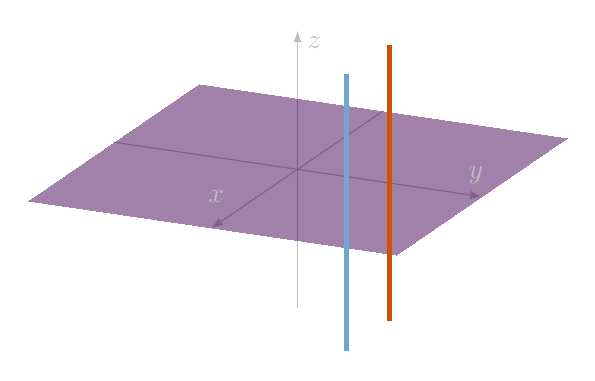
\begin{tikzpicture}
    \begin{axis}[
        axis lines = center,
        axis line style={-latex, gray!50},
        xlabel = {$x$},
        ylabel = {$y$},
        zlabel = {$z$},
        label style={gray!50},
        xmin=-2, xmax=2,
        ymin=-2, ymax=2,
        zmin=-2, zmax=2,
        ticks=none,
        view={115}{25},
        clip=false
    ]

        % Variety V(z): The xy-plane
        \addplot3[
            surf,
            opacity=0.5,
            colormap/viridis,
            domain=-2:2,
            domain y=-2:2,
            samples=2, % Simple plane only needs 2 samples
            shader=interp
        ] {0};

        % Variety V(x, y-1): Vertical line at (0, 1)
        % Drawn in two parts or with thick styling to stand out
        \addplot3[
            ultra thick,
            burntorange,
            domain=-2:2,
            samples y=0
        ] (0, 1, {x});
        
        % Variety V(x-1, y-1): Vertical line at (1, 1)
        \addplot3[
            ultra thick,
            iceberg,
            domain=-2:2,
            samples y=0
        ] (1, 1, {x});
    \end{axis}
\end{tikzpicture}
    \]
  \end{itemize}
\end{proof}

\begin{thebibliography}{99}
    \bibitem{DF04}
    D. S. Dummit και R. M. Foote, 
    \textit{Abstract algebra},
    third edition, Wiley, 2004. 
    \bibitem{Mal08}
    Μ. Μαλιάκας, 
    \textit{Εισαγωγή στην Μεταθετική Άλγεβρα}, 
    Εκδόσεις Σοφία, 2008.
\end{thebibliography}
\end{document}